%
% File acl2012.tex
%
% Contact: Maggie Li (cswjli@comp.polyu.edu.hk), Michael White (mwhite@ling.osu.edu)
%%
%% Based on the style files for ACL2008 by Joakim Nivre and Noah Smith
%% and that of ACL2010 by Jing-Shin Chang and Philipp Koehn

\documentclass[11pt]{article}
\usepackage{acl2012}
\usepackage{times}
\usepackage{latexsym}
\usepackage{amsmath}
\usepackage{multirow}
\usepackage{url}
\usepackage{graphicx}
\usepackage{booktabs}
\DeclareMathOperator*{\argmax}{arg\,max}
\setlength\titlebox{6.5cm}    % Expanding the titlebox

\title{Emotional Responses to Poetry}

\author{P. Thomas Barthelemy \\
  Computer Science\\
  Stanford University \\
  {\tt bartho@stanford.edu} \\\And
  Rob Voigt \\
  East Asian Studies \\
  Stanford University \\
  {\tt robvoigt@stanford.edu} \\\And
  Jean Y. Wu \\
  Symbolic Systems  \\
  Stanford University\\
  {\tt jeaneis@stanford.edu} \\}

\date{}

\begin{document}
\maketitle
\begin{abstract}
  This document contains the instructions for preparing a camera-ready manuscript for the proceedings of ACL2012. The document itself conforms to its own specifications, and is therefore an example of what your manuscript should look like. These instructions should be used for both papers submitted for review and for final versions of accepted papers. Authors are asked to conform to all the directions reported in this document.
\end{abstract}

\section{Introduction}

\paragraph{}
\emph{Poetry is when an emotion has found its thought and the thought has found words.}
\begin{flushright}
--- Robert Frost\\
\end{flushright}


Literature in general and poetry in particular present unique challenges for natural language understanding systems. Literary scholars often articulate the manner in which the primary purpose of literature is deviance, in some sense, from the common expectations we hold of human language. Raymond Chapman describes literature as ``the art that uses language,'' and Viktor Shklovskij notes that in poetry in particular we consistently find ``material obviously created to remove the automatism of perception.'' In Shklovskij's terms, literature effects a ``defamiliarization'' that surprises, delights, and moves to emotion in a way normal language does not.

It is fascinating that poetry is often able to concisely deliver a high emotional impact to its readership, and indeed this is an aspect of poetry that sets it apart from other genres of text. Literary interpretations of this characteristic of poetry have focused on highly contextual, semantic, and topical factors; for example, consider T.S. Eliot's concept of the "objective correlative" \cite{eliot}. Eliot proposes that emotion in poetry is generated by means of "a set of objects, a situation, [or] a chain of events which shall be the formula of that particular emotion," that is, by placing the reader at the center of an artfully described - and therefore richly imagined - context that would naturally generate such an emotion.

There is also a common emphasis in the literary community on "formal devices," including aspects of the structure of poetry as well as literary devices that poetry often employs, such as alliteration, rhyme, meter, and other forms of wordplay and creative use of language. [add a cite?] However, the explicit connection between such devices and emotiveness is no

Therefore, in this project we are interested in discovering the features of poetic texts that correlate highly with a strong emotional response.


\subsection*{Task}
This work focuses on emotional responses to poetry. For a given poem, we will attempt to identify and extract features which are capable of predicting a distribution over emotional categories seen in the comments responding to the poem. Our task can be divided into two phases: feature extraction for the purpose of describing poems and comment labelling. We will then use a MaxEnt classifier to predict emotional response distributions for new poems, and discuss which features contribute most significantly to these predictions.



\section{Related Work}

\newcite{kao2012computational} used computational methods to classify aesthetics of contemporary poetry. In particular, they analyzed diction, sound devices (rhyme, alliteration, and assonance), and imagery. As a proxy for a labeling poems as aesthetic or non-aesthetic, Kao and Jurafsky simply used the classes of professional versus amateur, which is expected to closely represent the former two categories with the advantage of having obvious labels.

Kao and Jurafsky hypothesized that diction would be important for classifying poetry. Poetic language is often �intentionally ambiguous�, attempting to capture multiple meanings simultaneously. Additionally, it is more likely to include uncommon �strange� words for the purpose of being distinguished. For this latter point, it is hypothesized that poetry would include more words with lower word frequencies. It was also hypothesized that poetry would utilize more varied vocabulary��varied� meaning including more word types, and avoiding the repeat of words. However, results showed that professional poets did not use more �strange� words; words used by professional poets were not significantly more unusual from words used by amateur poets. On the other hand, poets did use more distinct word types.

Additionally, it was observed that professional poets use more concrete words. Essentially, this could be viewed as a measure of imagery�imagery is conveyed through concrete details, and concrete details require non-abstract language. Similarly, professional poems were less likely to include psychological terms or positive/negative emotional terms, which further suggests that poets prefer to explain emotions via scenario description. In short, a professional poets follow the adage �show, don�t tell.�

Finally, with regard to form, professional poetry employs far fewer overt sound devices than does amateur poetry. So, though the findings of Tizhoosh et al. suggest that poetry is easily recognized by form, Kao and Jurafsky suggest that good poetry uses these cues far more sparingly. Further, though the perspective that the goal of poetry is to be distinguished (i.e. the poetry-as-deviance perspective) is weakened by the absence of strange words in poetry, it is revived in the observation that good contemporary poetry defies conventional poetic form.

\section{Dataset}
For this study, we propose a free-text to free-text framework for analysis. That is, we frame the problem as a classification task where each poem acts as a training example from which we extract a set of linguistic and poetic features. Each poem is then associated with the set of free-text responses to that poem from which we extract data to act as the poem's ``response label." Various implementations [wrong word? fix] of these response labels are described later in the paper.

\subsection*{Data Collection}
For a first pass at data collection, we ran a trial experiment on Amazon's Mechanical Turk service with five ten-line poems. We showed each poem to 20 Turkers and asked them to read and digest its contents. We then asked for them to provide a free-text response describing their personal, subjective emotional reaction to the poem. 

However, upon manual review of the results, we found them to be of roughly similar quality to comments provided on the website PoemHunter.com, and therefore changed our approach for data collection to web-scraping, to allow both for a larger dataset and a more varied selection of poems. We treat the comments for a given poem as our free-text responses for the purposes of this study.

We began by scraping the "Top 500 Poems" section of the website, comprised of poems by professional poets. Since there are many thousands of poems on the site and comments are relatively sparse, these poems offered a high density of comments for collection. It is not clear, however, how these "Top" poems were selected (it is evidently not based upon rating or number of comments), and so this selection has the potential to skew our results.

Therefore, we scraped an additional 25,000 poems from the site by following links to poets in the "Top 500 Poets" list. Since the distribution of comments is very sparse and scraping is a time-consuming process, we scraped and only use poems from this set with over 10 comments in response; this requirement cut down this additional data source to only approximately [do exact number?] 500 new poems, each with more than 10 comments.

\subsection*{Corpus Composition}

\section{Methodology}
Our task is quite generally defined as the prediction of a human response to poetry. To this end, we use features to describe the poems and their resulting comments. We use latter to capture the human response, and we use the former to predict the latter.

\subsection*{Poem Features}
% TODO: fix citations!
Poetic features are in part taken from \newcite{kao2012computational}, where they were used to analyze the asthetics of poetry, and Tizoosh et al, where they were used to classify poetry. We can divide them into three groups: orthography, sound device, and sentiment.

\emph{Orthographic Features}
Orthographic features capture the \emph{shape} of the poems. To decribe this, we used the following features: number of lines, number of stanzas, number of lines per stanzas, number of words per line, and type token ratio.

\emph{Sound Device Features}
Uniquely prevalent to poetry, sound device is a strong descriptive feature for both identifying poetry (Tizhoosh et al.) and classifying profession versus amatuer poetry. We used the CMU pronunciation dictionary, which maps words to phonemes.

In particular, we quantified perfect rhyme, slant rhyme, and alliteration. Perfect rhyme is defined as rhyme having the same ending vowel sound but differing consonant sound preceding it. Slant rhyme is defined as having the same ending consonant sound, but a different vowel sound preceding it. To simplify feature extraction, we avoid searching for particular rhyme schemes (e.g. aabb, ABAB), and simply check whether the ending word of a given sentence rhymes with the ending word of one of the previous two sentences. This ignores cases in which rhyme skips two lines, and would grossly underestimate the rhyming of, say, a Petrarchan Sonnet (abbaabbacdecde), though these rhyme schemes appear rarely.

We capture alliteration by counting the words within a fixed window having the same starting consonant sound. This is an approximation, as alliteration is rather defined as the repetition of stressed consonant sounds, which may include sounds occuring within a word.

Additionally and unlike \shortcite{kao2012computational} and Tizhoosh et al, we added features to quantify the proportion of nasals, fricatives, stops, and liquids. 

% TODO: how do we justify this again?

\subsection*{Comment Features}
We focus on two main ways of categorizing comment response: sentiment and diction.

\emph{Orthographic Features}
At first glance, there is a stark contrast between those comments that are thoughtful and lengthy and those comments that simply praise the poet in few words. Thus, we attempt to distinguish between these types of responses by counting the average response length (in words) and the type-token ratio.

As a technical note, we use the log of the average word length. Intuitively, this captures the notion that a difference in comment length of 10 and 15 is much larger than a difference in 50 and 55. As an additional technical note, we extract the type-token ratio for a particular poem's response by treating all comments as one document. Then, we sample 100 words from each response and calculate the type-token ratio for this. This offers a more principled way of comparing type-token ratios across differently sized documents.

\emph{Sentiment Features}
% TODO: citation of NRC?
It is predicted that human response will vary depending on the poems; some might elicit joy, others sadness. To this end, we attempt to measure the distribution and the magnitude of sentiment words. To measure the distribution of sentiment words, we use the NRC lexicon to associate given words with categories. For example, the word ``abacus'' is associated with the ``trust'' category. In all, there are 10 categories: anger, anticipation, disgust, fear, joy, negative, positive, sadness, surprise, and trust.

Additionally, we try to categorize the magnitude of the affect response by counting the frequency of affect words in a particular comment. We use the Linguistic Inquiry and Word Count (LIWC) dictionary to define affect words.


\section{Experiments}

\subsection{Predicting Sentiment Distribution}
Our first task was to predict the sentiment distribution of the poem responses. Performance would thus simply be based on the KL divergence of the predicted sentiment distribution and the actual distribution. This proved to be a difficult task, however, as our predicted distribution was no better than simply average distribution over all poems. Further analysis revealed that the word distributions were nearly identical across all poem responses, as shown in Figure~\ref{histogram}.

\begin{figure*}[ht]
\begin{center}
% \begin{align*}
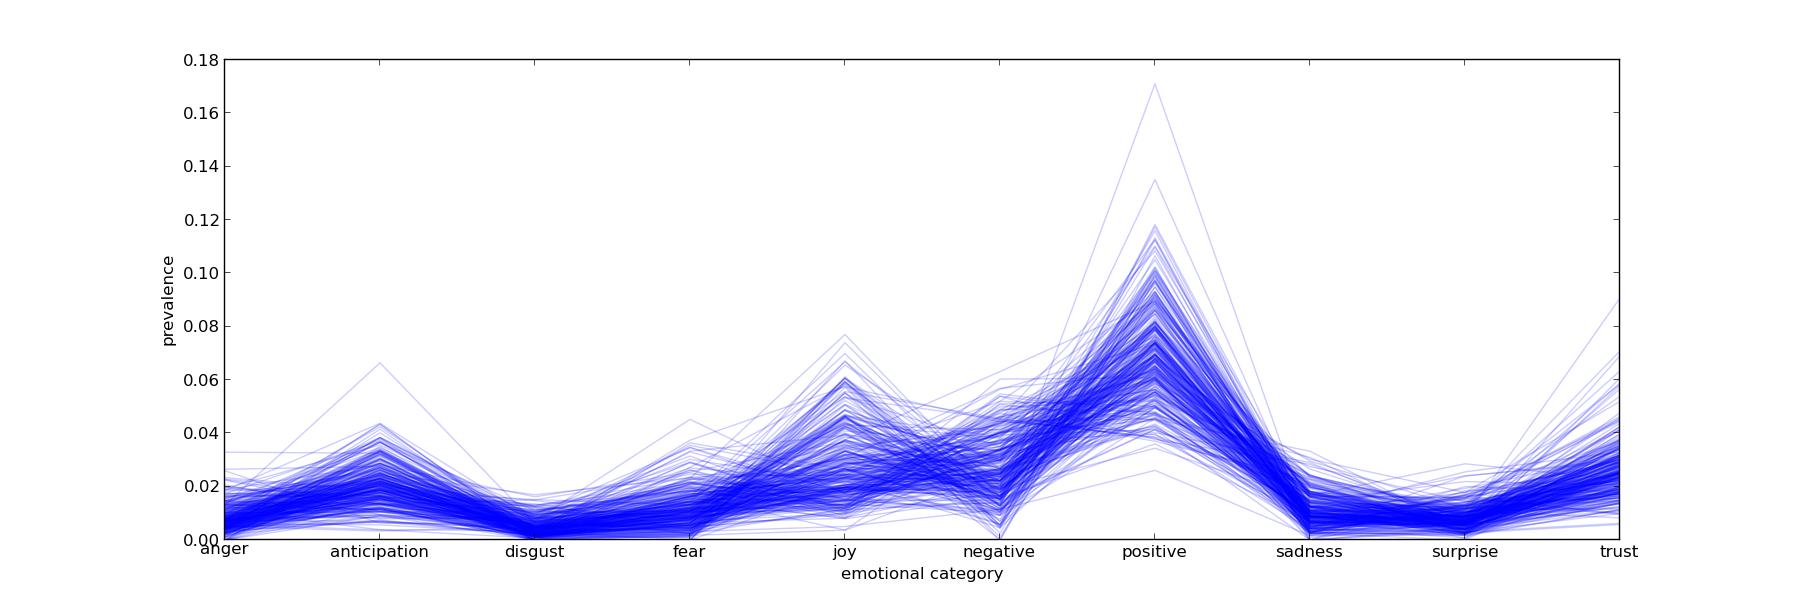
\includegraphics[scale=0.4]{../experiments/exp10.jpg}
% \end{align*}
\end{center}
\caption{A histogram of word distributions of the response for each poem. Here, each poem is represented by one line. The heavy overlap suggests that there is much similarity in the word distribution over comments.}
\label{histogram}
\end{figure*}

\section{Discussion}



\section{Future work}



\section*{Acknowledgments}

Do not number the acknowledgment section. Do not include this section when submitting your paper for review.


\bibliographystyle{acl}
\bibliography{bib}

\begin{thebibliography}{}
\bibitem[\protect\citename{Eliot}1921]{eliot}
T. S. Eliot.
\newblock 1921.
\newblock Hamlet and His Problems.
\newblock In {\em Sacred Wood}.
\newblock New York: Alfred A. Knopf.

\end{thebibliography}



\clearpage
\section*{Appendix}
\begin{table*}[th]%
%\vspace{-0.8cm}
\begin{center}
\scriptsize
\begin{tabular}{c @{\hspace{0pt}}  @{\hspace{15pt}}p{.88\textwidth}}
\toprule[.12em]\addlinespace
{\bf\small Category} & {\bf\small Words ordered by intensity (hight to low) } \\ \addlinespace
\midrule \addlinespace
anger & 
worthless	;
dreadful	;
disgusting	;
irritating	;
holocaust	;
horrible	;
annoyance	;
hate	;
depraved	;
hell	;
sucker	;
idiotic	;
disaster	;
bile	;
beating	;
abomination	;
bad	;
abhorrent	;
devastating	;
miserable	;
horrid	;
shoddy	;
atrocious	;
nasty	;
bitch	;
inexcusable	;
bomb	;
disgust	;
disdain	;
annoying	;
disappoint	;
revulsion	;
frustration	;
violence	;
cruelly	;
phony	;
unfulfilled	;
unlucky	;
intolerable	;
aggravating	;
ruined	;
suicidal	;
misery	;
agony	;
sin	;
irreconcilable	;
terrible	;
insulting	;
disease	;
evil	;
discord	;
disappointed	;
senseless	;
oppressive	;
bogus	;
despicable	;
delusional	;
horrific	;
assault	;
suffocation	;
violent	;
mournful	;
disgrace	;
villainous	;
arrogant	;
rejects	;
unhappy	;
frustrated	;
immorality	;
dissolution	;
punishing	;
guilty	;
hurt	;
infantile	;
insecure	;
abuse	;
spiteful	;
hiss	;
treachery	;
cancer	;
anger	;
obnoxious	;
vulgarity	;
jealousy	;
menace	;
limited	;
torture	;
deplorable	;
wreck	;
deceit	;
angry	;
idiocy	;
theft	;
satanic	;
incongruous	;
lagging	;
immaturity	;
menacing	;
teasing	;
resentment	;
inept	;
cruel	;
neglected	;
contempt	;
furious	;
shaky	;
terrorist	;
painful	;
catastrophe	;
dislike	;
turmoil	;
offended	;
complain	;
chaos	;
scare	;
cursing	;
contemptible	;
inappropriate	;
failing	;
lunacy	;
insignificant	;
dismay	;
grievous	;
alienation	;
sinner	;
insane	;
grumble	;
anguish	;
assassination	;
robbery	;
murderer	;
noisy	;
venomous	;
foul	;
insult	;
shoot	;
loathe	;
reject	;
leukemia	;
alienate	;
attack	;
pillage	;
offend	;
distressing	;
avarice	;
endless	;
crucifixion	;
argue	;
damn	;
incompetent	;
grating	;
antithesis	;
terrorism	;
indignation	;
lose	;
perverse	;
losing	;
repellent	;
bankruptcy	;
gore	;
rage	;
gibberish	;
offensive	;
lying	;
havoc	;
struggle	;
criticism	;
furiously	;
mad	;
wreak	;
ridiculous	;
pessimism	;
dupe	;
hateful	;
uncertain	;
loathsome	;
crushed	;
loss	;
dying	;
oblivion	;
murderous	;
molestation	;
devastation	;
bitterly	;
offense	;
damage	;
destructive	;
subversive	;
revolting	;
shun	;
stifled	;
unsettled	;
vengeance	;
fiend	;
overbearing	;
disservice	;
trickery	;
chaotic	;
bias	;
unsympathetic	;
confined	;
opium	;
hellish	;
selfish	;
suicide	;
disastrous	;
bloody	;
unpaid	;
misleading	;
anarchy	;
wasted	;
slap	;
indignant	;
profane	;
distracting	;
victim	;
dishonest	;
inhuman	;
choke	;
despair	;
hatred	;
scream	;
gang	;
controversial	;
hanging	;
horror	;
curse	;
darkness	;
victimized	;
poverty	;
sinister	;
collision	;
hurting	;
bully	;
difficulty	;
hostile	;
disillusionment	;
shooting	;
murder	;
depressed	;
lie	;
prisoner	;
cheat	;
crime	;
indifference	;
cranky	;
sabotage	;
steal	;
disturbance	;
obscenity	;
copycat	;
glaring	;
conflict	;
jealous	;
destruction	;
masochism	;
complaint	;
mob	;
imprisonment	;
demonic	;
distracted	;
politics	;
desert	;
yell	;
shortage	;
battle	;
punishment	;
bigoted	;
threatening	;
badness	;
manipulation	;
intractable	;
dishonor	;
sham	;
money	;
execution	;
warfare	;
dispossessed	;
intolerance	;
shot	;
awful	;
skewed	;
armed	;
warp	;
complicate	;
belittle	;
slavery	;
prejudice	;
willful	;
upset	;
discontent	;
delinquent	;
betray	;
confusion	;
threaten	;
abandoned	;
resentful	;
fuss	;
forsaken	;
moody	;
invade	;
frightful	;
gory	;
dabbling	;
fury	;
fear	;
vampire	;
melodrama	;
tension	;
sickening	;
lonely	;
treacherous	;
bickering	;
hood	;
egregious	;
insanity	;
attacking	;
outrage	;
hostage	;
reversal	;
enemy	;
scorn	;
profanity	;
cracked	;
fighting	;
perdition	;
detract	;
incendiary	;
broken	;
stone	;
assassin	;
fight	;
lynch	;
sly	;
malice	;
aftermath	;
brutal	;
illegal	;
condescension	;
obstacle	;
unruly	;
crazy	;
homicide	;
revolt	;
greed	;
thump	;
bout	;
cutting	;
crushing	;
revenge	;
rebel	;
disturbed	;
sarcasm	;
shiver	;
morbidity	;
sordid	;
combat	;
patter	;
massacre	;
injustice	;
killing	;
blame	;
kicking	;
conflagration	;
cruelty	;
violently	;
possessed	;
clashing	;
depravity	;
brutality	;
confront	;
claw	;
adversity	;
clash	;
strained	;
rejection	;
punitive	;
concealment	;
upheaval	;
cutthroat	;
reckless	;
pique	;
vicious	;
misunderstanding	;
force	;
punch	;
shrill	;
advocacy	;
caution	;
lunatic	;
ruinous	;
doomsday	;
carnage	;
betrayal	;
resent	;
torpedo	;
raging	;
harshness	;
deadly	;
tirade	;
death	;
wince	;
fatal	;
ruthless	;
expulsion	;
anarchist	;
morals	;
cacophony	;
opposed	;
unthinkable	;
brazen	;
bang	;
averse	;
boisterous	;
disobedience	;
paucity	;
threat	;
gall	;
tumult	;
antagonism	;
vent	;
intrusive	;
arguments	;
beast	;
savage	;
infidelity	;
scandalous	;
recklessness	;
disreputable	;
waffle	;
whip	;
contentious	;
deny	;
accused	;
ill	;
cross	;
slave	;
rating	;
row	;
mosque	;
rob	;
screwed	;
smack	;
screaming	;
compulsion	;
celebrity	;
shock	;
gun	;
harry	;
hating	;
lawyer	;
shriek	;
ridicule	;
soldier	;
moral	;
paralyzed	;
strike	;
domination	;
rivalry	;
cad	;
scar	;
court	;
boxing	;
delay	;
rape	;
invasion	;
deterioration	;
words	;
wound	;
versus	;
smash	;
payback	;
opera	;
inflict	;
rail	;
sneak	;
mistress	;
maniac	;
illicit	;
vote	;
divorce	;
storm	;
bloodshed	;
savagery	;
tree	;
youth	;
defense	;
polemic	;
argument	;
shell	;
react	;
flog	;
aggressive	;
latent	;
sentence	;
mug	;
penalty	;
cannon	;
bear	;
interminable	;
erupt	;
schizophrenia	;
bark	;
warrior	;
witch	;
madness	;
battery	;
defiance	;
demand	;
clamor	;
mangle	;
pound	;
sting	;
ransom	;
defiant	;
rebellion	;
warden	;
musical	;
provocation	;
rocket	;
kick	;
taunt	;
entangled	;
spine	;
lightning	;
prison	;
slash	;
convict	;
retribution	;
spat	;
frenzied	;
wireless	;
usurp	;
duel	;
aversion	;
retaliatory	;
stripped	;
deserve	;
smell	;
stab	;
suppression	;
tumultuous	;
dominate	;
mortality	;
brunt	;
raving	;
grim	;
tease	;
resistance	;
revolution	;
banger	;
blatant	;
bummer	;
evade	;
tolerate	;
simmer	;
grab	;
hoot	;
hardened	;
retaliation	;
distress	;
diatribe	;
shout	;
deranged	;
sizzle	;
criminal	;
contemptuous	;
sisterhood	;
cash	;
martial	;
ordeal	;
ferocious	;
diabolical	;
ferocity	;
feeling	;
frenetic	;
riot	;
challenge	;
crazed	;
unbridled	;
belt	;
provoking	;
spite	;
blasphemous	;
fits	;
mighty	;
involvement	;
explode	;
explosive	;
backbone	;
treat	;
blast	;
eviction	;
intolerant	;
disagree	;
hysterical	;
fierce	;
hit	;
sterling	;
intense	;
excite	;
honest	;
hot	;
playful	;
powerful	;


\\ \addlinespace
2 &
excellent performances ; 
amazing performance ; 
terrific performances ; 
A masterpiece ; 
masterful film ; 
wonderful film ; 
terrific performance ; 
masterful piece ; 
wonderful movie ; 
marvelous performances ; 
worst movie ; 
bad movie ; 
very bad ; 
shapeless mess ; 
worst thing ; 
tepid waste ; 
instantly forgettable ; 
bad film ; 
extremely bad ; 
complete failure ; 


\\\addlinespace\bottomrule[.12em]
\end{tabular}
%\vspace{-0.3cm}
\caption{Emotive words ordered by the intensity scores.}
\label{table:exPolarity}
\vspace{.4cm}
\end{center}
\end{table*}


>>>>>>> d51d3e3b4e21abd0b4474f78c064c4dc32a45866


\end{document}
